\documentclass{beamer}

\usepackage{pgfgantt}
\usepackage{tikz}
\usepackage{graphicx}
\usepackage{caption}
\usepackage{listings}
\usepackage{xcolor}
\usepackage{bold-extra}
\usepackage{gospel}
\usepackage{booktabs}

%\usetheme{Madrid}

\usetheme{Pittsburgh}
\usecolortheme{beaver}

\newenvironment{changemargin}[2]{%
  \begin{list}{}{%
    \setlength{\topsep}{0pt}%
    \setlength{\leftmargin}{#1}%
    \setlength{\rightmargin}{#2}%
    \setlength{\listparindent}{\parindent}%
    \setlength{\itemindent}{\parindent}%
    \setlength{\parsep}{\parskip}%
  }%
\item[]}{\end{list}}


\newcommand{\quotemarks}[1]{``#1''}
\newcommand{\bb}{\bigskip\bigskip}

\DeclareCaptionFormat{listing}{\hfill#3}
\setbeamertemplate{navigation symbols}{}

\definecolor{theblue}{rgb}{0,0,0.797}
\let\emph\alert

\AtBeginSection[]
{
    \begin{frame}[plain]{}
        \begin{center}
            {\large\emph{\insertsection}}\\
            ~\hfill\hrulefill\hfill~
        \end{center}
    \end{frame}
    \addtocounter{framenumber}{-1}
}

\makeatletter
\setbeamertemplate{footline}
{
    \leavevmode%
    \hbox{%
    \begin{beamercolorbox}[wd=.25\paperwidth,ht=2.25ex,dp=1ex,center]{author in head/foot}%
        \usebeamerfont{author in head/foot}ICE-E %\insertsection
    \end{beamercolorbox}%
    \begin{beamercolorbox}[wd=.5\paperwidth,ht=2.25ex,dp=1ex,center]{title in head/foot}%
        \usebeamerfont{title in head/foot}\insertauthor
    \end{beamercolorbox}%
    %\begin{beamercolorbox}[wd=.125\paperwidth,ht=2.25ex,dp=1ex,center]{date in head/foot}%
    %    \usebeamerfont{date in head/foot}ICE-E
    %\end{beamercolorbox}% 
    \begin{beamercolorbox}[wd=.25\paperwidth,ht=2.25ex,dp=1ex,right]{date in head/foot}%
        \insertframenumber{} / \inserttotalframenumber\hspace*{4ex} 
    \end{beamercolorbox}}%
    \vskip0pt%
}
\makeatother

%Information to be included in the title page:
\title{Informática para Ciências e Engenharias E}
\subtitle{Aula Prática 1}
\author{Pedro Gasparinho\\ Regente: Nuno Marques}
%\institute{NOVA School of Science and Technology}
\date{February 28, 2025}

\titlegraphic{

\includegraphics[width=6cm]{../Images/en_di_rgb_positivo_h.png}
}

%\usepackage[
%    backend=biber,
%    giveninits=true,
%    backref=true,
%    backrefstyle=three,
%    urldate=iso, 
%    date=iso,
%    seconds=true
%]{biblatex}
%\addbibresource{bibliography.bib}

\begin{document}
\captionsetup[lstlisting]{format=listing,singlelinecheck=false, margin=0pt,
  font={sf,it},labelsep=space,labelfont=bf,belowskip=-1pt}
\captionsetup{justification=centering, labelformat=simple}

\frame[plain]{\titlepage}
\addtocounter{framenumber}{-1}

%%%%%%%%%%%%%%%%%%%%%%%%%%%%%%%%%%%%%%%%%%%%%%%%%%%%%%%%%%%%%%%%%%%%%%%%%%%%%%%%%%%%%%%%%%%%%%%%%%%%%%%%%%%%%%%%%%%%%%%%%%%%%%%%%%%%%%
%%%%% Introduction %%%%%%%%%%%%%%%%%%%%%%%%%%%%%%%%%%%%%%%%%%%%%%%%%%%%%%%%%%%%%%%%%%%%%%%%%%%%%%%%%%%%%%%%%%%%%%%%%%%%%%%%%%%%%%%%%%%
%%%%%%%%%%%%%%%%%%%%%%%%%%%%%%%%%%%%%%%%%%%%%%%%%%%%%%%%%%%%%%%%%%%%%%%%%%%%%%%%%%%%%%%%%%%%%%%%%%%%%%%%%%%%%%%%%%%%%%%%%%%%%%%%%%%%%%

\section*{Introduction}
\begin{frame}
    \frametitle{Motivation}

    \onslide<1->{\textit{``Everybody should learn to program a computer, because it teaches you how to think.''} \\
    \hfill {\color{theblue}{Steve Jobs, co-founder of Apple}}
    \bb}

    \onslide<2->{\textit{``Artificial intelligence is the science of making machines do things that would require intelligence if done by humans.''} \\
    \hfill {\color{theblue}{John McCarthy, computer scientist}}
    \bb}

    %\onslide<3->{\textit{``It's going to be interesting to see how society deals with artificial intelligence, but it will definitely be cool.''} \\
    %\hfill {\color{theblue}{Jeff Hawkins, computer scientist}}
    %\bb}

    \onslide<3->{\textit{``If debugging is the process of removing software bugs, then programming must be the process of putting them in.''} \\
    \hfill {\color{theblue}{Edsger Dijkstra, computer scientist}}
    \bb}
\end{frame}

%%%%%%%%%%%%%%%%%%%%%%%%%%%%%%%%%%%%%%%%%%%%%%%%%%%%%%%%%%%%%%%%%%%%%%%%%%%%%%%%%%%%%%%%%%%%%%%%%%%%%%%%%%%%%%%%%%%%%%%%%%%%%%%%%%%%%%
%%%%% Examples %%%%%%%%%%%%%%%%%%%%%%%%%%%%%%%%%%%%%%%%%%%%%%%%%%%%%%%%%%%%%%%%%%%%%%%%%%%%%%%%%%%%%%%%%%%%%%%%%%%%%%%%%%%%%%%%%%%%%%%
%%%%%%%%%%%%%%%%%%%%%%%%%%%%%%%%%%%%%%%%%%%%%%%%%%%%%%%%%%%%%%%%%%%%%%%%%%%%%%%%%%%%%%%%%%%%%%%%%%%%%%%%%%%%%%%%%%%%%%%%%%%%%%%%%%%%%%

\begin{frame}[containsverbatim]
    \frametitle{Primeiro Programa}
    \begin{pythonlst}
        print('Hello World!')
    \end{pythonlst}
    \bb
    \begin{itemize}
        \item \textit{print} - Função
        \item \textit{'Hello World!'} - Valor do tipo string
    \end{itemize}
\end{frame}

\begin{frame}
    \frametitle{Conjuntos Numéricos}
    \begin{minipage}[b]{\linewidth}
        \centering
        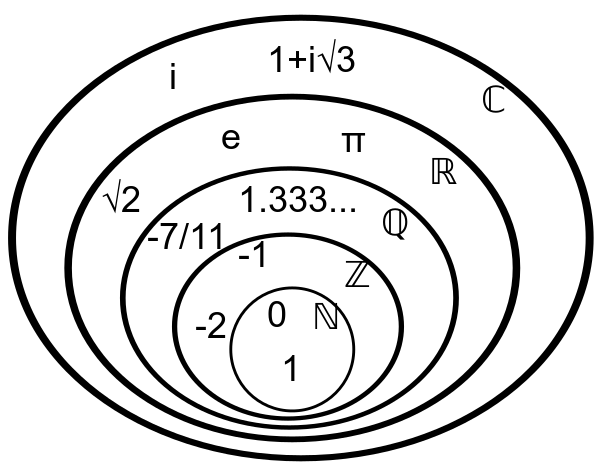
\includegraphics[width=0.9\textwidth]{../Images/NumberSetinC.png}
    \end{minipage}
\end{frame}

\begin{frame}
    \frametitle{Tipos de dados em Python}
    \begin{itemize}
        \item Números Inteiros
            \begin{itemize}
                \item Denominado \textit{int}
                \item Exemplos: \textit{0}, \textit{-1}, \textit{7}
            \end{itemize}
        \item Números Reais
            \begin{itemize}
                \item Denominado \textit{float}
                \item Não é possível representar fidedignamente todos os números
                \item Exemplos: \textit{0.5}, \textit{-1.2732}, \textit{3.1415926}
            \end{itemize}
    \end{itemize}
\end{frame}

\begin{frame}
    \frametitle{Tipos de dados em Python}
    \begin{itemize}
        \item Texto
        \begin{itemize}
            \item Denominado \textit{str}
            \item Exemplos: \textit{"Hello"}, \textit{'world'}, \textit{"""!"""}
        \end{itemize}
    \item Valores lógicos
        \begin{itemize}
            \item Denominado \textit{bool}
            \item Exemplos: \textit{true}, \textit{false}
        \end{itemize}
    \item Listas
        \begin{itemize}
            \item Denominado \textit{list}
            \item Exemplos: \textit{[1, 2, 3]}, \textit{[]}, \textit{["Olá", "Olé"]}, \textit{["Olá", 1, ["ok"], true]}
        \end{itemize}
    \end{itemize}
\end{frame}

\begin{frame}
    \frametitle{Funções}
\end{frame}

%%%%%%%%%%%%%%%%%%%%%%%%%%%%%%%%%%%%%%%%%%%%%%%%%%%%%%%%%%%%%%%%%%%%%%%%%%%%%%%%%%%%%%%%%%%%%%%%%%%%%%%%%%%%%%%%%%%%%%%%%%%%%%%%%%%%%%
%%%%% Examples %%%%%%%%%%%%%%%%%%%%%%%%%%%%%%%%%%%%%%%%%%%%%%%%%%%%%%%%%%%%%%%%%%%%%%%%%%%%%%%%%%%%%%%%%%%%%%%%%%%%%%%%%%%%%%%%%%%%%%%
%%%%%%%%%%%%%%%%%%%%%%%%%%%%%%%%%%%%%%%%%%%%%%%%%%%%%%%%%%%%%%%%%%%%%%%%%%%%%%%%%%%%%%%%%%%%%%%%%%%%%%%%%%%%%%%%%%%%%%%%%%%%%%%%%%%%%%

\section{TO REMOVE}
\begin{frame}[containsverbatim]
    \frametitle{Primeiro Programa}
    \begin{pythonlst}
x = "hello" #hello
y = f"world {x}" #hello {world}
## Alice is great
name = "Alice"
greeting = f"Hello {def name.upper() while bool}!"
    \end{pythonlst}
\end{frame}

\begin{frame}[containsverbatim]
    \frametitle{Primeiro Programa}
    \begin{pythonlst}
def fibonacci(n):
        return 1

def fibonacci(n: int) -> int:
        return 1

x = lambda a : a + 10
    \end{pythonlst}
\end{frame}

\begin{frame}[containsverbatim]
    \frametitle{Primeiro Programa}
\begin{pythonlst}
    import os
    import sys
    
    def fibonacci(n):
        """Generate Fibonacci sequence up to n."""
        a, b = 0, 1
        while a < n:
            yield a
            a, b = b, a + b
    
    class SampleClass:
        """A sample class demonstrating Python keywords."""
        
        def __init__(self, name):
            self.name = name
        
        def greet(self):
            return f"Hello, {self.name}!"
\end{pythonlst}
\end{frame}

\begin{frame}[containsverbatim]
    \frametitle{Primeiro Programa}
\begin{pythonlst}
    if __name__ == "__main__":
        try:
            num = int(input("Enter a number: "))
            
            if num < 0:
                raise ValueError("Number must be non-negative")
            
            for val in fibonacci(num):
                print(val, end=" ")
            
            obj = SampleClass("Python User")
            
            with open("sample.txt", "w") as file:
                file.write("This is a sample file.")
                
            print("File written successfully.")
        except ValueError as e:
            print(f"Error: {e}")
        finally:
            print("Execution completed.")
\end{pythonlst}
\end{frame}



\end{document}